\documentclass[a4paper,11pt]{ltjsarticle}

\usepackage{amsmath,amssymb,mathtools,bm}
\usepackage{graphicx}
\usepackage{xcolor}
\usepackage[numbers,sort&compress]{natbib}
\usepackage{url}
\usepackage{hyperref}
\hypersetup{
  colorlinks=true,
  allcolors=blue!50!black,
  bookmarksnumbered=true,
  pdftitle={小売の店舗分布と二点相関関数},
}

\graphicspath{{../docs/figures/}}

\newcommand{\repourl}{https://github.com/inuverse44/retail-cosmology}
\newcommand{\code}[1]{\texttt{#1}}

\title{小売の店舗分布と二点相関関数\\
  \large Coles と Woolworths に Landy--Szalay 推定量を当てる}
\author{Inuverse}
\date{\today}

\begin{document}
\maketitle
\tableofcontents

\section{動機}

オーストラリアの小売は Coles と Woolworths の二社が大きな割合を占める。
日本と比べて商品の入れ替わりが遅いこと、物流拠点から店舗までの距離が長いことが、店舗の配置に表れているかを調べたい。
ここでは店舗の座標を銀河の位置に見立て、宇宙論で銀河の分布を測るときの二点相関関数を当てる。

\section{二点相関関数}

面密度 $n$ の点過程で、面積要素 $\delta S_1$, $\delta S_2$ に一点ずつ見つかる確率を
\begin{equation}
  \delta P = n^2 \bigl[1 + \xi(r)\bigr]\, \delta S_1\, \delta S_2
  \label{eq:xi-def}
\end{equation}
と書き、$\xi(r)$ を二点相関関数と呼ぶ。
点が互いに独立に撒かれていれば（ポアソン過程）$\xi = 0$ である。

\section{推定量}

データ $n_d$ 点と、同じ領域に一様に撒いたランダム $n_r$ 点を用意する。
距離のビンごとに、データ同士の対の数 $DD$、データとランダムの対の数 $DR$、ランダム同士の対の数 $RR$ を数え、
それぞれ全対数 $n_d(n_d-1)/2$, $n_d n_r$, $n_r(n_r-1)/2$ で割ったものを $dd$, $dr$, $rr$ とする。
推定量は次の 4 つを実装した。
\begin{align}
  \hat\xi_{\mathrm{N}}  &= \frac{dd}{rr} - 1, &
  \hat\xi_{\mathrm{DP}} &= \frac{dd}{dr} - 1, \\
  \hat\xi_{\mathrm{H}}  &= \frac{dd\, rr}{dr^2} - 1, &
  \hat\xi_{\mathrm{LS}} &= \frac{dd - 2\,dr + rr}{rr}.
  \label{eq:estimators}
\end{align}
$\hat\xi_{\mathrm{DP}}$ は Davis と Peebles \cite{DavisPeebles1983}、$\hat\xi_{\mathrm{H}}$ は Hamilton \cite{Hamilton1993}、
$\hat\xi_{\mathrm{LS}}$ は Landy と Szalay \cite{LandySzalay1993} による。
実装は \href{\repourl/blob/main/crates/retail-cosmology/src/lib.rs}{\nolinkurl{crates/retail-cosmology/src/lib.rs}} にある。

\section{toy model}

相関のない点で、推定量が $0$ のまわりに散ることを確かめる。
単位正方形に一様に $2000$ 点を撒いてデータとし、別に $8000$ 点を撒いてランダムとした（図~\ref{fig:toy}）。
\begin{figure}[htbp]
  \centering
  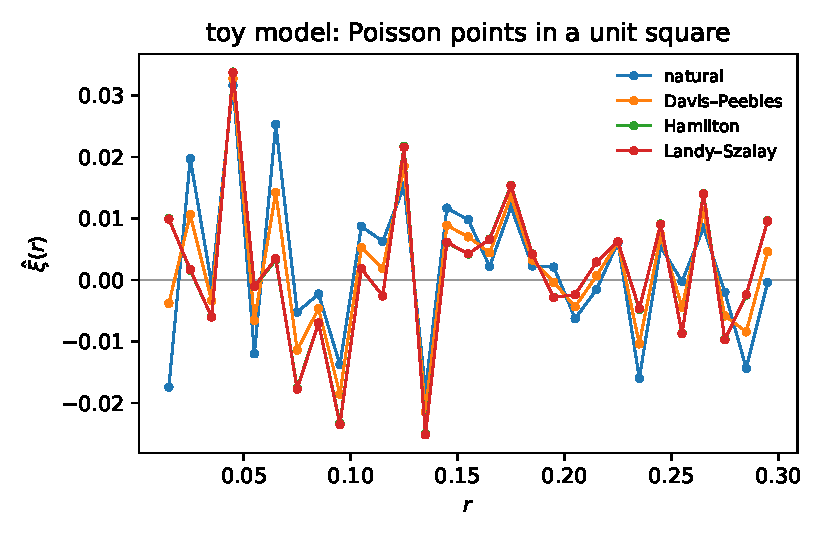
\includegraphics[width=0.8\linewidth]{toy_poisson.pdf}
  \caption{単位正方形のポアソン点に対する 4 つの推定量。
    \code{cargo run --release --bin toy} の出力を \code{scripts/plot\_toy.py} で描いた。}
  \label{fig:toy}
\end{figure}

\section{店舗データ}

未定。取得元・取得日・ライセンスと、距離（大円距離）とランダムカタログ（オーストラリアの陸地に一様か、人口で重みをつけるか）の決め方をここに書く。

\bibliographystyle{unsrtnat}
\bibliography{references}

\end{document}
